
\documentclass[a4paper,12pt]{article} % тип документа
\usepackage{tikz}
\usetikzlibrary{plotmarks}
% The data files, written on the first run.
\begin{filecontents}{div_soft.data}
#MOPS 	Power [mW]
1.33E-02	10.403432
1.33E-01	12.53108
2.66E-01	14.90265
3.99E-01	17.22483
5.31E-01	19.58292
6.64E-01	21.89876
7.97E-01	24.44624
9.30E-01	26.6708
\end{filecontents}

\begin{filecontents}{div_ciu.data}
# MOPS 	Power [mW]
4.35E-02	9.562436
4.35E-01	10.845494
8.69E-01	12.24356
1.30E+00	13.66974
1.74E+00	15.13008
2.17E+00	16.57845
2.61E+00	17.97894
3.04E+00	19.41534
\end{filecontents}

\begin{filecontents}{div_ciu_oscar.data}
#MOPS 	Power [mW]
8.57E-01	11.255013
9.99E-01	11.4804
1.14E+00	11.718
1.29E+00	11.9916
1.64E+00	12.65854
2.00E+00	13.308
2.64E+00	14.484
3.85E+00	16.8
\end{filecontents}

\begin{filecontents}{div_ciu_oscar_extrapolated.data}
# MOPS 	Power [mW]
4.28E+00	17.56312023
5.71E+00	20.21127914
7.14E+00	22.85943805
8.57E+00	25.50759696
9.99E+00	28.15575587
\end{filecontents}
% report, book
\binoppenalty=10000
\relpenalty=10000
%  Русский язык

\usepackage[T2A]{fontenc}			% кодировка
\usepackage[utf8]{inputenc}			% кодировка исходного текста
\usepackage[english,russian]{babel}	% локализация и переносы


% Математика
\usepackage{amsmath,amsfonts,amssymb,amsthm,mathtools} 


\usepackage{wasysym}

\title{Лабораторная работа 1.1.6 по курсу \\ "Общая физика"  \\ 
\vspace{0.2cm}
\vspace{4.5cm}
 \LARGE{\textbf{ИЗУЧЕНИЕ ЭЛЕКТРОННОГО ОСЦИЛЛОГРАФА}}\vspace{5.5cm}}
\date{14.09.2018}
\usepackage{tikz}
\author{\vspace{0.2cm}Баринов Леонид}

\begin{document} % начало документа

\maketitle

\newpage


\textbf{Цель работы: } Изучение устройства осциллографа и механизмов его работы

\textbf{Оборуднование} Осциллограф, генераторы электрических сигналов, соединительные кабели


\section{Теоретические сведения}

Осциллограф - регистрирующий прибор, в котором исследуемое напряжение (сигнал) преобразуется в видимый на экране график изменения напряжения во времени.

Основной частью электронного осциллографа, определяющей его\\ важнейшие технические характеристики, является электронно-лучевая трубка (ЭЛТ).

Трубка представляет собой стеклянную откачанную до высокого вакуума колбу, в которой расположены: подогреватель катода, катод, модулятор, первый (фокусирующий) анод, второй (ускоряющий) анод, горизонтально и вертикально отклоняющие пластины, третий (ускоряющий) анод, экран.

\section{Ход работы}
\subsection{Наблюдение периодического сигнала от генератора и измерение его частоты}
Получаем на экране осциллографа устойчивую картину периодического (синусоидального) сигнала, подаваемого с генератора, и с помощью горизонтальной шкалы экрана осциллографа проводим измерение периода и частоты сигнала.
\begin{center}
\begin{table}[!h]
\begin{tabular}{|c|c|c|c|c|c|c|c|}
\hline
fзг,Гц & T, дел & мс/дел   & T,мc  &$\delta T$ & f  &$\delta f$ & f - fзг, Гц \\ \hline
20     & 5,0   & 10,00 & 50,00 & 1,000  & 20,00   &   0,40    & 0,00        \\ \hline
513    & 4,0   & 0,50 & 2,00  & 0,050 & 500,00  &     12,50   & -13,00      \\ \hline
1012   & 5,0   & 0,20 & 1,00  & 0,020& 1000,00 &    20,00    & -12,00      \\ \hline
1916   & 5,2   & 0,10 & 0,52 & 0,010& 1923,08 &     36,98   & 7,08        \\ \hline
5502   & 3,6   & 0,05 & 0,18 & 0,005& 5555,56 &   154,32     & 53,56       \\ \hline
\end{tabular}
\caption{Наблюдение периодического сигнала от генератора и измерение его частоты}
\end{table}
\end{center}
Цена деления осциллографа равна $0,2$дел. Погрешность осциллографа равна половине цены деления. При перемножениее $0,1$дел на количество секунд на одно деление получаем $\delta T$. 
Частоту сигнала $f$ находим по формуле $f = 1/T$. $\delta f$ вычисляем по формуле:
\[\delta f = \frac{\delta T}{T}f\]
Из результатов, зансесенных в таблицу видно, что $f$зг $\simeq f$ c учетом погрешности. 
\subsection{Измерение амплитуды сигнала}
\righthyphenmin=2
\hfuzz=2.5pt
С помощью вертикальной шкалы экрана осциллографа измеряем отношение максимальной и минимальной амплитуд напряжений $Umax/Umin$ которые способен выдавать генератор.
{\tolerance=400

}

Измерения проводяться при частоте $f = 1$кГц
{\raggedright

}
$Umax = 11,000 (2.2$дел$\times  5B/$дел)
{\raggedright

}
$Umin = 0,066 (3.3$дел$\times  0,02B/$дел)
{\raggedright

}
Выражаем отношение максимального и минимального уровней сигнала $\beta_{21}$ в \textit{децибелах} [дБ]
\[ \beta_{21} = 20 lg{\frac{Umax}{Umin}}\]
$\beta_{21} \approx 44,44$дБ

\subsection{Измерение амплитудно-частотной характеристики осциллографа}
\textit{Амплитудно-частотной} характеристикой (АЧХ) измерительного прибора называют зависимость амплитуды измеряемого сигнала от частоты сигнала, подаваемого на вход. Проведем измерения АЧХ  осциллографа во всем диапазоне рабочих частот генератора.

Изменяя частоту 	$f$ звукого генератора во всем доступном диапазоне, исследуем зависимость отношения амплитуды сигнала на осциллографе $U(f)$ к исходной $U_0(=3$дел) в зависимости от частоты:
\[K(f) = \frac{U(f)}{U_0}\]\\
В области частот, где $K$ отличается от единицы, проведем подробные измерения $K(f)$. Измерения амплитудно-частотных характеристик $K(f)$ проведем для одного из каналов осциллографа при открытом (DC, $\simeq $) и при закрытом (АС, $\sim $) входе. Результаты занесем в таблицу

\begin{table}[ht]
\begin{tabular}{|l|c|c|c|c|c|c|}
\hline
$f$, Гц        & 0,028  & 1,920 & 19    & \textbf{1009}  & 3471  & 4624  \\ \hline
$lg f$         & -1,553 & 0,283 & 1,279 & \textbf{3,004} & 3,540 & 3,665 \\ \hline
$2U_{AC}$, дел    & 6,0    & 6,0   & 6,0   & \textbf{6,0}   & 6,0   & 6,0   \\ \hline
$K_{AC} = U_{AC}/Uo$ & 1,00   & 1,00  & 1,00  & \textbf{1,00}  & 1,00  & 1,00  \\ \hline
$2U_{DC}$, дел    & 6,0    & 6,0   & 6,0   & \textbf{6,0}   & 6,0   & 6,0   \\ \hline
$K_{DC} = U_{DC}/Uo$ & 1,00   & 1,00  & 1,00  & \textbf{1,00}  & 1,00  & 1,00  \\ \hline
\end{tabular}

\end{table}

\begin{table}[h]
\begin{tabular}{|l|c|c|c|c|c|}
\hline
$f$, Гц     & 5549  & 60300 & 1978000 & 2740000 & 5334000 \\ \hline
$lg f$        & 3,744 & 4,780 & 6,296   & 6,438   & 6,727   \\ \hline
$2U_{AC}$   & 6,0   & 6,0   & 5,9     & 5,8     & 5,7     \\ \hline
$K_{AC} = U_{AC}/Uo$ & 1,00  & 1,00  & 0,98    & 0,97    & 0,95    \\ \hline
$2U_{DC}$, дел    & 6,0   & 6,0   & 5,9     & 5,8     & 5,7     \\ \hline
$K_{DC} = U_{DC}/Uo$ & 1,00  & 1,00  & 0,98    & 0,97    & 0,95    \\ \hline
\end{tabular}
\end{table}

Построим в единых осях графики зависимостей коэффициента ослабления сигнала от частоты в лографмическом масштабе по частоте $K_{AC}(lg f)$ и $K_{DC} (lg f)$%.
\begin{figure}[!h]
\begin{center}
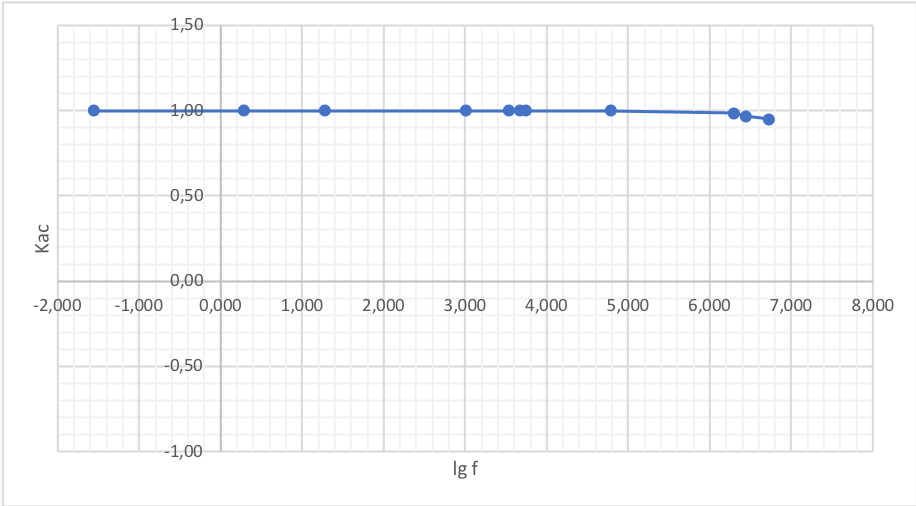
\includegraphics[width=1\textwidth]{1}
\end{center}
\caption{$K_{AC}(lg f)$ } \label{dz1}


\end{figure}
\begin{figure}[!h]
\begin{center}
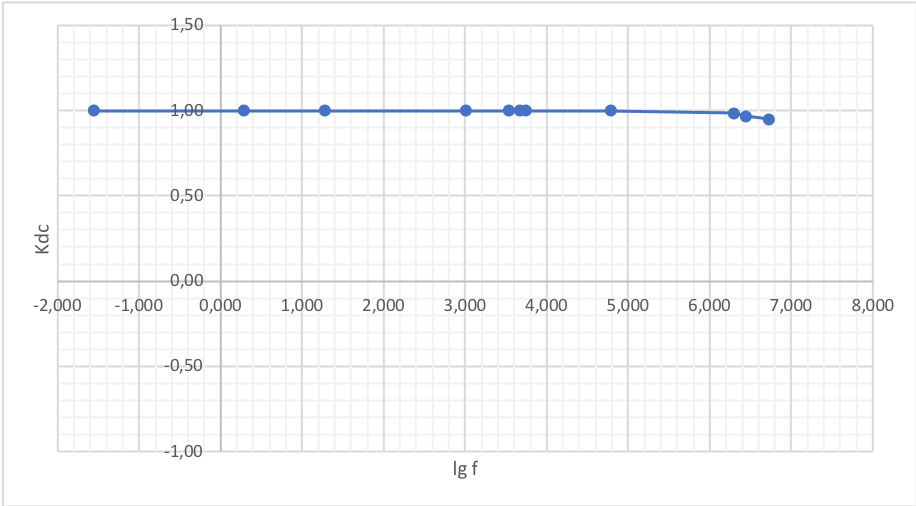
\includegraphics[width=1\textwidth]{2}
\end{center}
\caption{$K_{DC}(lg f)$ } \label{dz2}
\end{figure}
\newpage
АЧХ канала в разных разных режимах - горизонтальная линия. При значительном увеличении частоты наблюдается небольшое искажение АЧХ.
\subsection{Измерение разности фазово-частотных характеристик каналов осциллографа}
\textit{Фазово-частотной характеристикой} (ФЧХ) называют зависимость разности фаз входного и выходного сигналов от частоты. Проведем измерение разности фаз, возникающей при подаче одного и того же сигнала на разные каналы осциллографа, в зависимости от частоты сигнала.

При подаче на взаимно перпендикулярные отклоняющие пластины двух синусоидальных сигналов траектория луча на экране осциллографа представляет собой эллипс и может быть в общем виде описана уравнениями

\begin{equation}\label{1}
\begin{aligned}
x(t) = A_x sin(\omega t + \varphi_x), && y(t) = A_y sin(\omega t + \varphi_y)
\end{aligned}
\end{equation}

Разность фаз $\Delta\varphi = \varphi_y- \varphi_x$ можно выразить, положив в \eqref{1} $\omega t = -\varphi_x$, после чего получаем
\[sin |\Delta\varphi| = \left|\frac{y_0}{A_y}\right|\],\\
где $y_0 = y|_{x=0}$ - отклонение луча по вертикали в момент, когда его абсцисса равна нулю; $A_y$ - амплитуда колебаний по оси $y$. Тогда возможные значения разности фаз:
\begin{equation}\label{2}
\begin{aligned}
|\Delta\varphi| = arcsin \left|\frac{y_0}{A_y}\right|
\end{aligned}
\end{equation}\\
или
\begin{equation}\label{3}
\begin{aligned}
|\Delta\varphi| = \pi - arcsin \left|\frac{y_0}{A_y}\right|.
\end{aligned}
\end{equation}\\
При этом, если эллипс наклонен вправо, то угол $\Delta\varphi$ лежит в интервале $[-\pi/2; \pi/2]$	- имеет место формула \eqref{2}; если эллипс налонен влево, то $\Delta\varphi \in [\pi/2; \pi]\cup[-\pi; -\pi/2]$ - необходимо использовать формулу \eqref{3}. Результаты измерений занесем в таблицу:
\begin{table}[!h]
\begin{tabular}{|c|c|c|c|c|c|}
\hline
$f$, Гц   & $lg f$  & $|2y_{0}|$, дел & $|2A_{y}|$, дел & $arcsin|\frac{y_{0}}{Ay}|$, рад & $\Delta\varphi$, рад \\ \hline
32   & 1,509 & 0,1        & 2,2        & 0,045              & 0,045         \\ \hline
266   & 2,424 & 0,0        & 2,2        & 0,000              & 0,000         \\ \hline
1044    & 3,019 & 0,0        & 2,2        & 0,000              & 0,000         \\ \hline
169400  & 5,229 & 0,2        & 2,2        & 0,091              & 0,091         \\ \hline
354700  & 5,550 & 0,4        & 2,2        & 0,183              & 0,183         \\ \hline
536000  & 5,729 & 0,6        & 2,2        & 0,276              & 0,276         \\ \hline
768000  & 5,885 & 0,8        & 2,2        & 0,372              & 0,372         \\ \hline
915000  & 5,961 & 1,0        & 2,2        & 0,472              & 0,472         \\ \hline
1116000 & 6,048 & 1,2        & 2,2        & 0,577              & 0,577         \\ \hline
1309000 & 6,117 & 1,4        & 2,2        & 0,690              & 0,690         \\ \hline
1536000 & 6,186 & 1,6        & 2,2        & 0,814              & 0,814         \\ \hline
1875000 & 6,273 & 1,8        & 2,1        & 1,030              & 1,030         \\ \hline
2248000 & 6,352 & 2,0        & 2,0        & 1,571              & 1,571         \\ \hline
2458000 & 6,391 & 2,0        & 2,0        & 1,571              & 1,571         \\ \hline
2644000 & 6,422 & 1,8        & 2,0        & 1,120              & 2,022         \\ \hline
2783000 & 6,445 & 1,6        & 2,0        & 0,927              & 2,214         \\ \hline
2960000 & 6,471 & 1,4        & 2,0        & 0,775              & 2,366         \\ \hline
3433000 & 6,536 & 0,8        & 2,0        & 0,412              & 2,730         \\ \hline
4036000 & 6,606 & 0,7        & 2,0        & 0,358              & 2,784         \\ \hline
4227000 & 6,626 & 0,6        & 2,0        & 0,305              & 2,837         \\ \hline
4639000 & 6,666 & 0,2        & 2,0        & 0,100              & 3,041         \\ \hline
5341000 & 6,728 & 0,4        & 2,0        & 0,201              & 2,940         \\ \hline
\end{tabular}
\end{table}

\begin{figure}[!h]
\begin{center}
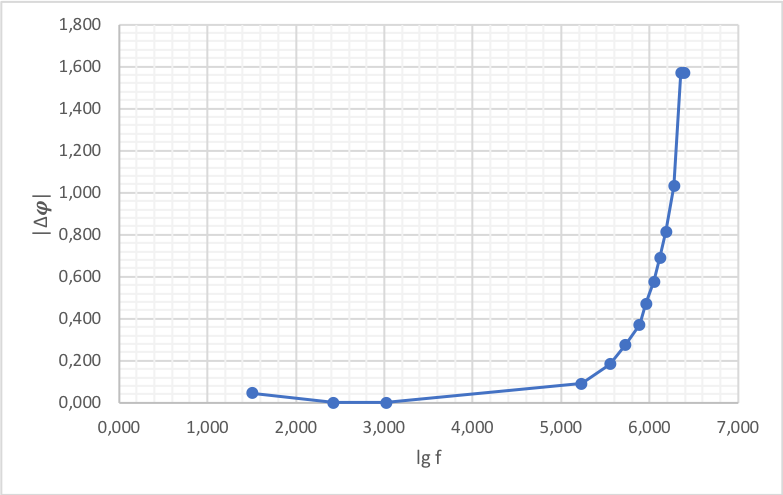
\includegraphics[width=1\textwidth]{3}
\end{center}
\caption{$|\Delta\varphi|(lg f)$  } \label{dz3}
\end{figure}
\newpage
При возрастании $f$ возрастает $|\Delta\varphi|$


\subsection{Наблюдение фигур Лиссажу и измерение частоты}

Подаем на вход каналов $X$ и $Y$ осциллографа сигналы с двух разных звуковых генераторов. Устанавливаем приблизительно одинаковые частоты генераторов. Изменяя $f_x$, получаем устойчивые фигуры для нескольких целочисленных отношений частот.
\begin{figure}[!h]
\begin{center}
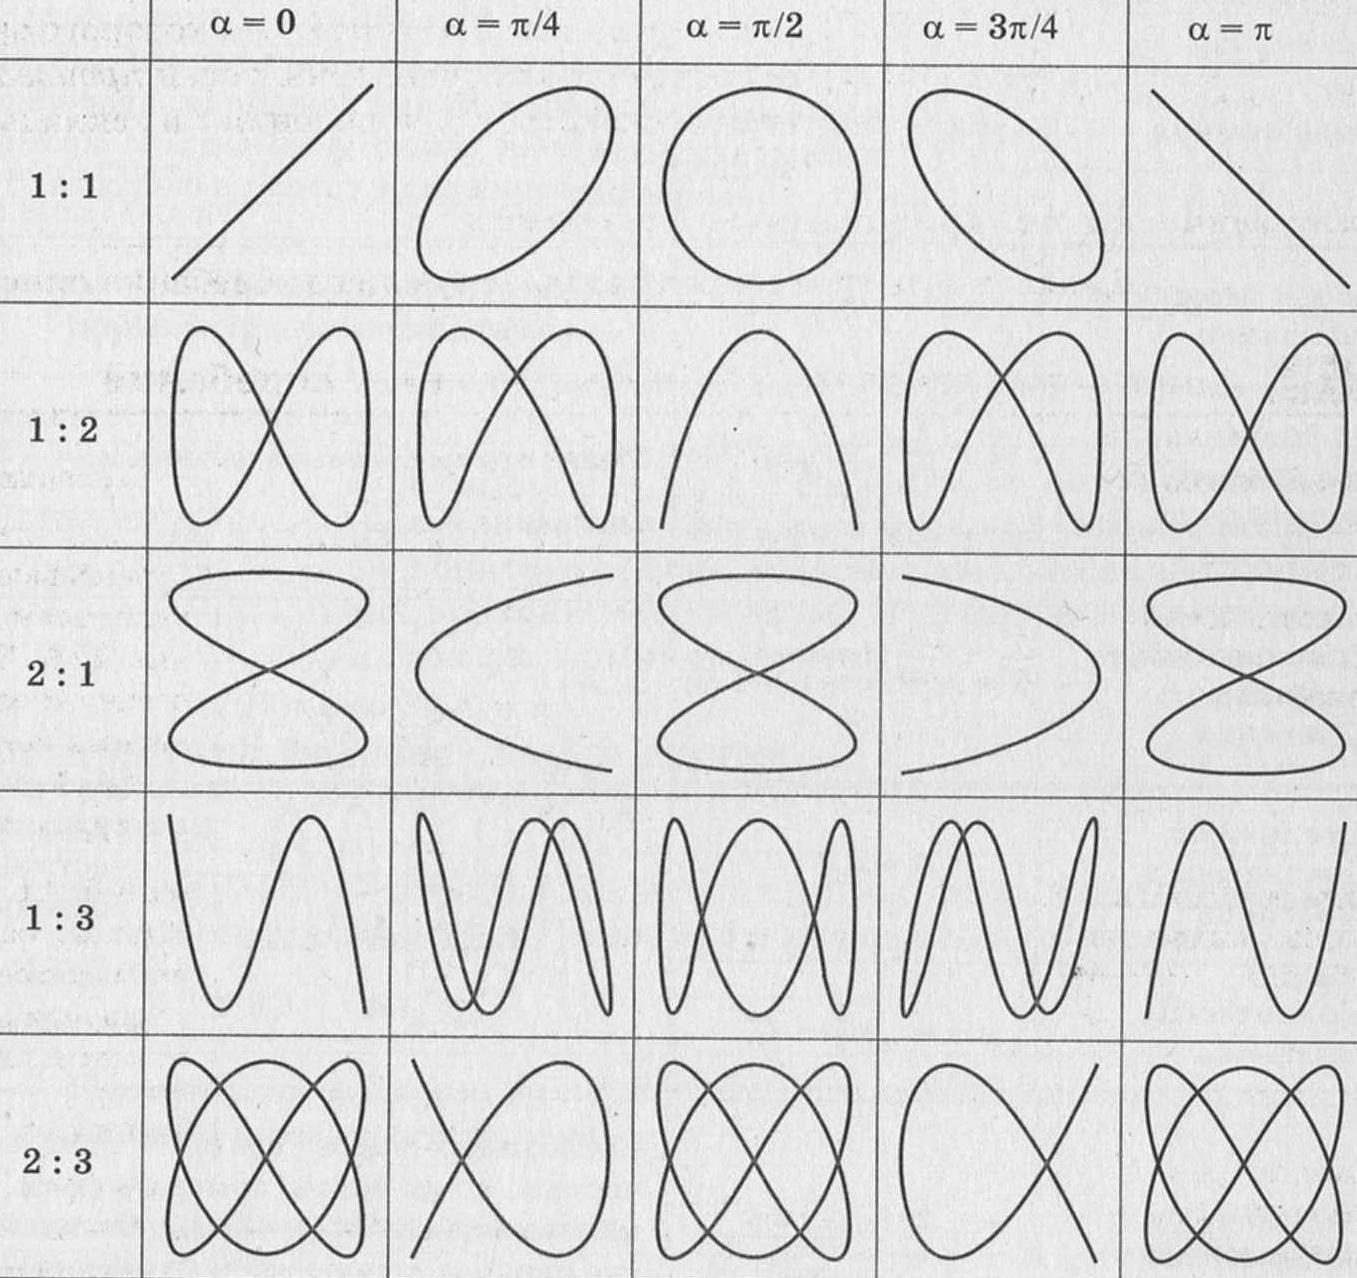
\includegraphics[width=0.7\textwidth]{5}
\end{center}
\caption{Фигуры Лиссажу для колебаний одинаковой амплитуды. $\alpha = \Delta\varphi$} \label{dz3}
\end{figure}

\begin{table}[h]
\begin{tabular}{|c|c|c|}
\hline
$f_y$, Гц & $f_x$, Гц & $f_x/f_y$ \\ \hline
79,3   & 79,1   & 1,00  \\ \hline
2040   & 4080   & 0,50  \\ \hline
297,6  & 99,1   & 3,00  \\ \hline
2010   & 1008   & 1,99  \\ \hline
202    & 303    & 0,67  \\ \hline
\end{tabular}
\end{table}
\newpage
\section{Вывод}
В этой работе мы узнали основные компоненты и органы управления осциллографа. Провели серию измерений и наблюдений различных физических величин с его помощью и проанализировали полученные данные.  

\begin{tikzpicture}[y=.2cm, x=.7cm,font=\sffamily]
 	%axis
	\draw (0,0) -- coordinate (x axis mid) (10,0);
    	\draw (0,0) -- coordinate (y axis mid) (0,30);
    	%ticks
    	\foreach \x in {0,...,10}
     		\draw (\x,1pt) -- (\x,-3pt)
			node[anchor=north] {\x};
    	\foreach \y in {0,5,...,30}
     		\draw (1pt,\y) -- (-3pt,\y) 
     			node[anchor=east] {\y}; 
	%labels      
	\node[below=0.8cm] at (x axis mid) {MOPS};
	\node[rotate=90, above=0.8cm] at (y axis mid) {Power [mW]};

	%plots
	\draw plot[mark=*, mark options={fill=white}] 
		file {div_soft.data};
	\draw plot[mark=triangle*, mark options={fill=white} ] 
		file {div_ciu.data};
	\draw plot[mark=square*, mark options={fill=white}]
		file {div_ciu_oscar.data};
	\draw plot[mark=square*]
		file {div_ciu_oscar_extrapolated.data};  
    
	%legend
	\begin{scope}[shift={(4,4)}] 
	\draw (0,0) -- 
		plot[mark=*, mark options={fill=white}] (0.25,0) -- (0.5,0) 
		node[right]{soft};
	\draw[yshift=\baselineskip] (0,0) -- 
		plot[mark=triangle*, mark options={fill=white}] (0.25,0) -- (0.5,0)
		node[right]{ciu};
	\draw[yshift=2\baselineskip] (0,0) -- 
		plot[mark=square*, mark options={fill=white}] (0.25,0) -- (0.5,0)
		node[right]{ciu + oscar};
	\draw[yshift=3\baselineskip] (0,0) -- 
		plot[mark=square*, mark options={fill=black}] (0.25,0) -- (0.5,0)
		node[right]{ciu + oscar extrapolated};
	\end{scope}
\end{tikzpicture}

\end{document} % конец документа
